\documentclass[border=0.8ex,svgnames,tikz]{standalone}
\usepackage{amsmath,mathtools}
\usepackage{fontspec}
\setmainfont{Source Serif 4}
\setsansfont{Source Sans 3}
\setmonofont{Source Code Pro}
\usetikzlibrary{positioning}
\begin{document}
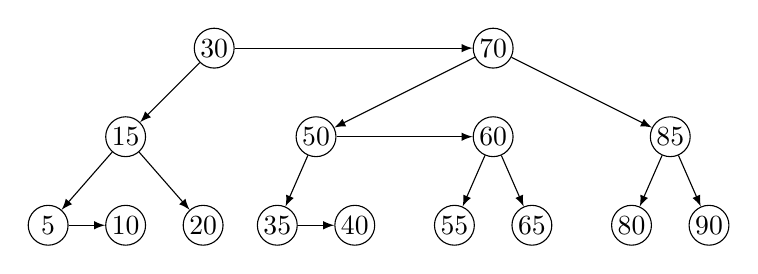
\begin{tikzpicture}[
  level distance=3.2em,
  every node/.style={draw,circle,inner sep=0.1ex,minimum size=1.44em},
  level 1/.style={sibling distance=6.4em},
  level 2/.style={sibling distance=2.8em},
  edge from parent/.style={draw=none},
  every path/.style={draw,>=latex},
  ]
  \node(n30){30}
  child{
    node(n15){15}
    child{ node(n5){5} }
    child{ node(n10){10} }
    child{ node(n20){20} }
  }
  child[missing];
  \node[right=8.6em of n30](n70){70}
  child{
    node(n50){50}
    child{ node(n35){35} }
    child{ node(n40){40} }
  }
  child{
    node(n60){60}
    child{ node(n55){55} }
    child{ node(n65){65} }
  }
  child{
    node(n85){85}
    child{ node(n80){80} }
    child{ node(n90){90} }
  };
  \path[->]
  (n30) edge (n15)
  (n15) edge (n5)
  (n5) edge (n10)
  (n15) edge (n20)
  (n30) edge (n70)
  (n70) edge (n50)
  (n50) edge (n35)
  (n35) edge (n40)
  (n50) edge (n60)
  (n60) edge (n55)
  (n60) edge (n65)
  (n70) edge (n85)
  (n85) edge (n80)
  (n85) edge (n90);
\end{tikzpicture}
\end{document}
